% Currículo de João Gabriel Salvador Paiva
% Vaga: Desenvolvedor Backend Python Júnior — byx (remoto, BR)
% Layout de coluna única, texto 100% selecionável, sem tabelas nem caixas de texto,
% para não quebrar a extração de texto por ATS.
\documentclass[10.5pt,a4paper]{article}

\usepackage[T1]{fontenc}
\usepackage[utf8]{inputenc}
\usepackage[brazil]{babel}
\usepackage{lmodern}
\usepackage[margin=1.5cm,top=1.2cm,bottom=1.2cm]{geometry}
\usepackage{graphicx}
\usepackage{enumitem}
\usepackage{titlesec}
\usepackage{xcolor}
\usepackage[hidelinks]{hyperref}
\usepackage{microtype}
\usepackage{needspace}

\definecolor{azul}{HTML}{14375A}

\hypersetup{
  pdftitle={Joao Gabriel Salvador Paiva - Desenvolvedor Backend Python Junior},
  pdfauthor={Joao Gabriel Salvador Paiva},
  pdfsubject={Curriculo - Desenvolvedor Backend Python Junior - byx},
  pdfkeywords={Python, Django, FastAPI, API REST, microsservicos, PostgreSQL, NoSQL, Redis,
  RabbitMQ, Celery, Docker, AWS, Git, testes automatizados, PyTest, CI/CD, GitHub Actions,
  observabilidade, Clean Code, SOLID, DDD, design patterns, Scrum, backend}
}

\pagestyle{empty}
\setlength{\parindent}{0pt}
\setlist[itemize]{leftmargin=3.6mm,itemsep=1pt,topsep=2pt,parsep=0pt,label=\textbullet}

\titleformat{\section}{\bfseries\large\color{azul}}{}{0em}{}[\vspace{-1.2ex}\rule{\linewidth}{0.6pt}]
\titlespacing{\section}{0pt}{2.2ex}{1.2ex}

\newcommand{\cargo}[4]{%
  \Needspace*{5\baselineskip}%
  \textbf{#1} \textnormal{---} #2 \hfill \textnormal{#3}\\
  \textit{\small #4}\vspace{0.4ex}
}

\begin{document}

%% ---------- Cabeçalho ----------
\begin{minipage}[c]{0.78\textwidth}
\raggedright
{\LARGE\bfseries\color{azul} João Gabriel Salvador Paiva}\\[0.6ex]
{\large Desenvolvedor Backend Python}\\[0.9ex]
\small
Campina Grande – PB, Brasil (disponível para trabalho remoto)\\
\href{mailto:joaogabrielsalvadorpaiva@gmail.com}{joaogabrielsalvadorpaiva@gmail.com} $\cdot$ +55 (83) 98863-6734\\
\href{https://github.com/Ilusinusmate}{github.com/Ilusinusmate} $\cdot$
\href{https://www.linkedin.com/in/joao-gabriel-salvador-paiva-805283286}{linkedin.com/in/joao-gabriel-salvador-paiva} $\cdot$
\href{https://ilusinusmate.github.io/Ilusinusmate/}{ilusinusmate.github.io/Ilusinusmate}
\end{minipage}\hfill
\begin{minipage}[c]{0.2\textwidth}
\raggedleft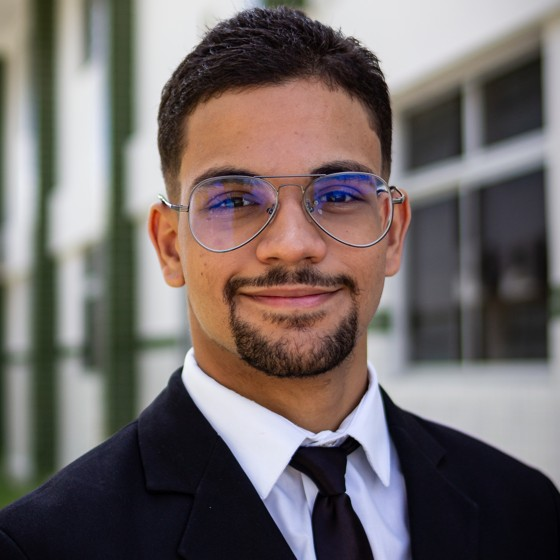
\includegraphics[width=2.7cm]{foto.jpg}
\end{minipage}

%% ---------- Resumo ----------
\section*{Resumo}
Desenvolvedor backend com quase 3 anos de experiência profissional em \textbf{Python}, atuando com
\textbf{Django} e \textbf{FastAPI} na construção de \textbf{APIs REST}, \textbf{microsserviços} e
integrações entre sistemas. Experiência com \textbf{PostgreSQL}, bancos \textbf{NoSQL},
\textbf{Redis}, filas assíncronas (\textbf{RabbitMQ}, \textbf{Celery}), \textbf{Docker},
\textbf{AWS} e \textbf{CI/CD}, escrevendo código testável orientado a \textbf{Clean Code},
\textbf{SOLID} e \textbf{DDD}. Backend de aplicações em produção com mais de 50 mil usuários ativos.
Estudante de Ciência da Computação na UFCG e residente em TIC no VIRTUS-CC/UFCG, com pesquisa
publicada sobre uso de LLMs em Engenharia de Software.

%% ---------- Competências ----------
\section*{Competências técnicas}
\textbf{Linguagens:} Python, Dart, JavaScript, TypeScript, SQL, C\\
\textbf{Backend:} Django, Django REST Framework, FastAPI, Flask, APIs REST, microsserviços,
autenticação, integrações entre sistemas\\
\textbf{Dados:} PostgreSQL, SQL, bancos NoSQL, Redis, MinIO, modelagem de dados\\
\textbf{Mensageria e assincronia:} RabbitMQ, Celery, filas assíncronas, CronJobs\\
\textbf{Infraestrutura:} Docker, AWS (S3, CloudFront), Railway, Render, Nginx, Linux\\
\textbf{Qualidade:} PyTest, mocks, testes automatizados, code review, Clean Code, SOLID, DRY, DDD,
design patterns\\
\textbf{Engenharia:} Git, GitHub Actions, CI/CD, observabilidade (OpenTelemetry, Grafana, logging),
documentação técnica, Scrum/Kanban, sistemas distribuídos

%% ---------- Experiência ----------
\section*{Experiência profissional}

\cargo{Logon Informática}{Mobile \& Backend Developer}{jan/2025 -- atual}{Software house de
sistemas de gestão para educação, administração pública e outros setores}
\begin{itemize}
  \item Desenvolvo e mantenho \textbf{microsserviços em Python/FastAPI} que sustentam o app
        \textit{Central da Escola}, com mais de \textbf{50 mil usuários ativos}.
  \item Implementei comunicação assíncrona entre serviços com \textbf{RabbitMQ} e armazenamento de
        objetos com \textbf{MinIO}, reduzindo acoplamento entre os módulos do produto.
  \item Lidero o setor de desenvolvimento mobile: planejamento, code review, releases em Android e
        iOS, logging e \textbf{CI/CD}.
  \item Escrevo a documentação técnica de APIs e serviços e faço a mediação entre times internos e
        integrações com sistemas de terceiros.
\end{itemize}

\cargo{Empório Sertanejo}{Desenvolvedor Backend --- líder técnico}{dez/2023 -- set/2025}{Franquia de
varejo de especiarias; SaaS proprietário de ERP, PDV e e-commerce}
\begin{itemize}
  \item Desenvolvi em \textbf{Django/Python} um SaaS integrando \textbf{ERP, PDV e e-commerce},
        com \textbf{PostgreSQL} e \textbf{Docker}, usado na operação diária de vendas e estoque.
  \item \textbf{Liderei 3 desenvolvedores}, definindo padrões de código, revisões e prioridades de
        entrega junto ao cliente.
  \item Implantei \textbf{testes automatizados com PyTest} e mocks, \textbf{CI/CD com GitHub
        Actions} e \textbf{observabilidade} com OpenTelemetry e Grafana para investigar erros em
        homologação e produção.
  \item Construí integrações e rotinas assíncronas (\textbf{CronJobs}, Pipedream, Mailgun) e
        publiquei os ativos estáticos em \textbf{AWS S3 + CloudFront}.
\end{itemize}

\cargo{VIRTUS-CC / Softex (UFCG)}{Residente em TIC --- pesquisador do grupo ISE}{nov/2025 --
atual}{Programa de residência em software de 1 ano: 240h de capacitação + imersão prática}
\begin{itemize}
  \item Aprovado em \textbf{1º lugar} no processo seletivo (\textbf{96/100} na prova de títulos e
        \textbf{100/100} na entrevista).
  \item Formação em Engenharia de Software I e II, \textbf{metodologias ágeis}, IoT, machine
        learning e design thinking, com projetos em squad multidisciplinar.
  \item Pesquisa no grupo \textbf{Intelligent Software Engineering}: avaliação de LLMs aplicados a
        qualidade de requisitos e engenharia de software ágil, com artigo aceito no
        \textbf{XP 2026} (Springer LNBIP).
\end{itemize}

\cargo{Animalesko}{Desenvolvedor Backend (voluntário)}{abr/2024 -- set/2024}{Startup social de apoio
a animais de rua}
\begin{itemize}
  \item Projetei a arquitetura backend do aplicativo com foco em baixo consumo de recursos, e
        documentei as decisões técnicas para o time.
\end{itemize}

\cargo{IFPB (CNPq / LAPLIN)}{Pesquisador bolsista e professor de Python}{2023 -- 2024}{Laboratório de
Análise e Processamento de Linguagem Natural}
\begin{itemize}
  \item Bolsista de pesquisa em processamento de linguagem natural, com liderança do grupo discente
        em dois projetos e publicações em eventos nacionais.
  \item Ministrei aulas de \textbf{Python} para cerca de 60 alunos, com material próprio e
        experimento comparando o aprendizado com e sem apoio de IA.
\end{itemize}

%% ---------- Projetos ----------
\section*{Projetos}
\begin{itemize}
  \item \textbf{pdfa-parser} --- biblioteca Python open source, publicada no \textbf{PyPI}, que
        converte PDFs para o padrão \textbf{PDF/A} e valida a conformidade automaticamente
        (GhostScript e VeraPDF), com APIs síncrona e assíncrona, CLI e execução em contêiner:
        \href{https://pypi.org/project/pdfa-parser}{pypi.org/project/pdfa-parser}
  \item \textbf{Contratexto} --- jogo web multiplayer em \textbf{FastAPI} com \textbf{WebSocket} e
        similaridade semântica (spaCy/NLP), com processamento em \textbf{fila assíncrona} para
        isolar o custo do modelo da requisição do usuário:
        \href{https://contratexto.onrender.com}{contratexto.onrender.com}
  \item \textbf{Corretor ONHB} --- aplicativo em Flutter, feito a pedido de professores do IFPB,
        que corrige automaticamente as provas da Olimpíada Nacional em História do Brasil.
\end{itemize}

%% ---------- Formação ----------
\section*{Formação}
\textbf{Bacharelado em Ciência da Computação} --- Univ. Federal de Campina Grande (UFCG)
\hfill jan/2025 -- 2030\\
\textbf{Técnico Integrado} --- Instituto Federal da Paraíba (IFPB) \hfill mar/2022 -- dez/2024\\
\textbf{Formação complementar} --- Python Backend Developer e Flutter Specialist (DIO)

%% ---------- Extras ----------
\section*{Publicações e prêmios (seleção)}
\begin{itemize}
  \item \textbf{8 trabalhos científicos} publicados sobre IA, LLMs e Engenharia de Software, entre
        eles \textit{Evaluating the Quality of User Stories: An Extended Comparative Study of
        Multiple LLMs and Rule-Based Tools} (XP 2026, Springer LNBIP, 2º autor) e artigos no
        \textbf{WEI 2025} e \textbf{WICS 2024} (Sociedade Brasileira de Computação).
  \item \textbf{Melhor resumo expandido} da modalidade Iniciação Científica e Tecnológica --- TIC
        no \textbf{5º SIMPIF} (2023).
  \item \textbf{Campeão da Olimpíada Paraibana de Informática} (2023), \textbf{ouro} na categoria
        Avançado Júnior (2026) e finalista da Olimpíada Brasileira de Informática (2023).
\end{itemize}

\section*{Idiomas}
Português (nativo) $\cdot$ Inglês (avançado --- leitura, escrita e comunicação profissional)
$\cdot$ Libras (intermediário) $\cdot$ Espanhol (aprendendo)

\end{document}
